%%% Ne pas modifier jusqu'à la ligne 25
\documentclass[a4paper,12pt]{book}
\usepackage[utf8]{inputenc}
\usepackage[french]{babel}
%%\usepackage{CJK}
\usepackage{yhmath}
\usepackage[left=2cm,right=2cm,top=3cm,bottom=2cm, headheight=1.5cm,headsep=1.5cm]{geometry}
%%\usepackage{CJKutf8}
\usepackage{amsfonts}
\usepackage{mathrsfs}
\usepackage{amsmath,amsfonts,amssymb,dsfont}
\usepackage{graphicx}
\usepackage{subfigure}
\usepackage{enumitem}		%\enumerate-resume
\usepackage[colorlinks=true,unicode={true},hyperindex=false, linkcolor=blue, urlcolor=blue]{hyperref}
\newcommand{\myref}[1]{\ref{#1} page \pageref{#1}}

\addto\captionsfrench{\def\tablename{Tableau}}  %légendes des tableaux
\renewcommand\thesection{\Roman{section}~-~} 
\renewcommand\thesubsection{\Roman{section}.\Alph{subsection}~-~} 
\renewcommand\thesubsubsection{\Roman{section}.\Alph{subsection}.\arabic{subsubsection}~-~} 

\newcommand{\conclusion}[1]{\newline \centerline{\fbox{#1}}}

\setcounter{secnumdepth}{3}
\parindent=0pt

\usepackage{fancyhdr}
\pagestyle{fancy}

\lhead{SJTU-ParisTech} 
%%%%%%%%%%%%%%%%%%%%%%%%%%%%%%%%%%
\chead{DM}
\rhead{Daniel 518261910024}
\begin{document}

\renewcommand{\labelitemi}{$\blacktriangleright$}
\renewcommand{\labelitemii}{$\bullet$}


\section{Exercice 1 : Manipulations sur les bornes inférieures et supérieures}
\subsection{}
Soit $(a,b) \in (A \cup B)^2$, on va distinguer deux cas:
\begin{itemize}
    \item S'il existe $p \in A$, $q \in B$ tels que $d(a,b)\leq d(p,q)$, alors pour tout
    $c \in A$, $d \in B$ on a 
    $$
    d(a,b)\leq d(p,q) \leq d(p,c)+d(c,d)+d(d,q) 
    $$
    car $(c,p) \in A^2$, $(d,q) \in B^2$, par la définition de borne supérieur, on a donc 
    $$
    d(a,b)-d(c,d) \leq d(p,c)+d(d,q)\leq diam(A)+diam(B)
    $$
    indépendant du choix de $(a,b)\in (A \cup B)^2$, on peut passer à la limite de cette inégalité, on obtient 
    $$
    diam(A \cup B)-d(c,d)\leq diam(A)+diam(B)
    $$
    donc 
    $$
    diam(A \cup B)-(diam(A)+diam(B)) \leq d(c,d)
    $$
    indépendant de choix du $(c,d)\in A\times B$, on peut passer à la limite de cette inégalité, on obtient 
    $$
    diam(A \cup B)- (diam(A)+diam(B)) \leq d(A,B)
    $$
    Finalement, 
    $$
    diam(A \cup B) \leq d(A,B)+diam(A)+diam(B)
    $$
    \item S'il n'existe pas $p \in A$, $q \in B$ tels que $d(a,b)\leq d(p,q)$, c'est à dire 
    $(a,b) \in A^2$ ou $(a,b) \in B^2$ et donc $diam(A \cup B)= diam(A)$ ou $diam(A \cup B)= diam(B)$, 
    on a bien 
    $$
    diam(A \cup B)\leq diam(A)+diam(B)+d(A,B)
    $$
\end{itemize}
En tout cas, on a $\boxed{diam(A \cup B)\leq diam(A)+diam(B)+d(A,B)}$

\subsection{}
Soient $(x,y) \in E^2$, alors il existe une suite $(u_n)_{n \in \mathbb{N}}$ de A telle que $d(y,u_n)\xrightarrow[n \to +\infty]{}d(y,A)$, 

Soit $n \in \mathbb{N}$, par inégalité triangulaire,  on a $d(x,u_n)-d(y,u_n)\leq d(x,y)$. Donc 
$$d(x,A)-d(y,u_n)\leq d(x,u_n)-d(y,u_n)\leq d(x,y)$$

On peut passer à la limite de cette inégalité, on obtient
$$
d(x,A)-d(y,A)\leq d(x,y)
$$
De même, on a aussi $d(y,A)-d(x,A)\leq d(x,y)$

Finalement, on a donc $\boxed{\forall (x,y) \in E^2, d(x,y) \geq |d(x,A)-d(y,A)|}$
\subsection{}
\begin{itemize}
    \item Par définition, $A \subset \overline{A}$, donc $\{(x,a), a\in A\}\subset \{(x,a),a \in \overline{A}\}$, 
    donc $\{d(x,a), a\in A\}\subset \{d(x,a),a \in \overline{A}\}$, on a donc 
    $$
    d(x,\overline{A})=inf\{d(x,a),a \in \overline{A}\} \leq inf\{d(x,a), a\in A\}=d(x,A)
    $$
    \item Soit $a \in \overline{A}$, par définition, il existe une suite $(u_n)_{n \in \mathbb{N}}$ de $A$ tel que $u_n \xrightarrow[n \to +\infty]{}a$, on a 
    $d(x,u_n)\xrightarrow[n \to +\infty]{}d(x,a)$. Par la définition de borne inférieure, on a $\forall n \in \mathbb{N}$, $d(x,u_n) \geq d(x,A)$. 
    Donc $d(x,a) \geq d(x,A)$, ce qui est indépendant du choix de $a$. On peut passer à la limite de cette inégalité, donc $d(x,\overline{A}) \geq d(x,A)$
\end{itemize}
Par double inégalité, on a $\boxed{d(x,\overline{A}) = d(x,A)}$

\section{Exercice 2}
\begin{itemize}
    \item On suppose que $k \geq \sqrt{2}$, on va montrer $F_k$ est un fermé de $(\mathbb{R}^2, \Vert\cdot\Vert_2)$.
    
    Soit $x \in F_k$, alors il existe $a \in \mathbb{N}^*$, tel que $x \in BF((\frac{1}{a},\frac{1}{a}),\frac{k}{a})$. Et on a 
    \begin{align*}
    \Vert x,(1,1)\Vert_2&\leq \Vert x,(\frac{1}{a},\frac{1}{a})\Vert_2+\Vert (\frac{1}{a},\frac{1}{a}),(1,1)\Vert_2\\
    & \leq \frac{k}{a}+\sqrt{2}(1-\frac{1}{a})\\
    &=\sqrt{2}+\frac{k-\sqrt{2}}{a}
    \end{align*}
    Car $a \in \mathbb{N}^*$ et $k \geq \sqrt{2}$, on a donc $\frac{k-\sqrt{2}}{a}\leq k-\sqrt{2}$, donc 
    $$
    \Vert x,(1,1)\Vert_2 \leq \sqrt{2}+k-\sqrt{2} \leq k
    $$
    donc $x \in BF((1,1),k)$, donc $F_k \subset BF((1,1),k)$. 

    D'autre part, on a clairement $ BF((1,1),k)  \subset F_k$, donc $F_k = BF((1,1),k)$ qui est un fermé de $(\mathbb{R}^2, \Vert\cdot\Vert_2)$
    % Soit $((x_n,y_n))_{n \in \mathbb{N}}$ une suite de $F_k$ qui converge dans $\mathbb{R}^2$, alors il existe $(x,y) \in \mathbb{R}^2$ tel que $(x_n,y_n) \xrightarrow[n \to +\infty]{}(x,y)$, 
    % donc on a $\Vert(x_n,y_n),(x,y)\Vert \xrightarrow[n \to +\infty]{}0$, donc $x_n\xrightarrow[n \to +\infty]{}x$, $y_n\xrightarrow[n \to +\infty]{}y$. Comme $(x_n,y_n) \in F_k$, alors il exist 
    % $a \in \mathbb{N}^*$ tel que 
    % $$
    % \Vert(x_n,y_n),\left(\frac{1}{a},\frac{1}{a}\right)\Vert=\sqrt{\left(x_n-\frac{1}{a}\right)^2+\left(y_n-\frac{1}{a}\right)^2}=\frac{\sqrt{2}}{a}\leq \frac{k}{a}
    % $$
    % par la continuité des fonctions $x \mapsto x^2$ et $x\mapsto \sqrt{x}$, on en déduit que 
    % $$
    % \sqrt{\left(x-\frac{1}{a}\right)^2+\left(y-\frac{1}{a}\right)^2}=\Vert(x,y),\left(\frac{1}{a},\frac{1}{a}\right)\Vert=\frac{\sqrt{2}}{a}\leq \frac{k}{a}
    % $$
    
    Donc lorsque $k \geq \sqrt{2}$, $F_k$ est un fermé de $(\mathbb{R}^2, \Vert\cdot\Vert_2)$.
    \item Soit $k < \sqrt{2}$, on peut définir la suite $(u_n)_{n \in \mathbb{N}^*}$, 
    telle que $\forall n \in \mathbb{N}^*$, $u_n=(\frac{1}{n}-\frac{k}{\sqrt{2}n},\frac{1}{n}-\frac{k}{\sqrt{2}n})$. La suite converge vers $(0,0)$, et on a 
    $$\forall n \in \mathbb{N}^*, \Vert u_n,(\frac{1}{n},\frac{1}{n})\Vert=\Vert(\frac{k}{\sqrt{2}n},\frac{k}{\sqrt{2}n})\Vert=\frac{k}{n}$$
    
    Donc $\forall n \in \mathbb{N}^*$, $u_n \in BF((\frac{1}{n},\frac{1}{n}),\frac{k}{n}) \subset F_k$
    
    Mais $ \forall a \in \mathbb{N}^*$ , $\Vert(0,0),(\frac{1}{a},\frac{1}{a})\Vert=\frac{\sqrt{2}}{a}>\frac{k}{a}$, donc 
    $(0,0) \notin F_k$, $F_k$ n'est pas un fermé de $(\mathbb{R}^2, \Vert\cdot\Vert_2)$

\end{itemize}
Finalemnt, on a $F_k$ est fermé si et seulement si $\boxed{k \geq \sqrt{2}}$
\section{Exercice 3}
\subsection{}
\begin{figure}[h]
    \begin{center}
    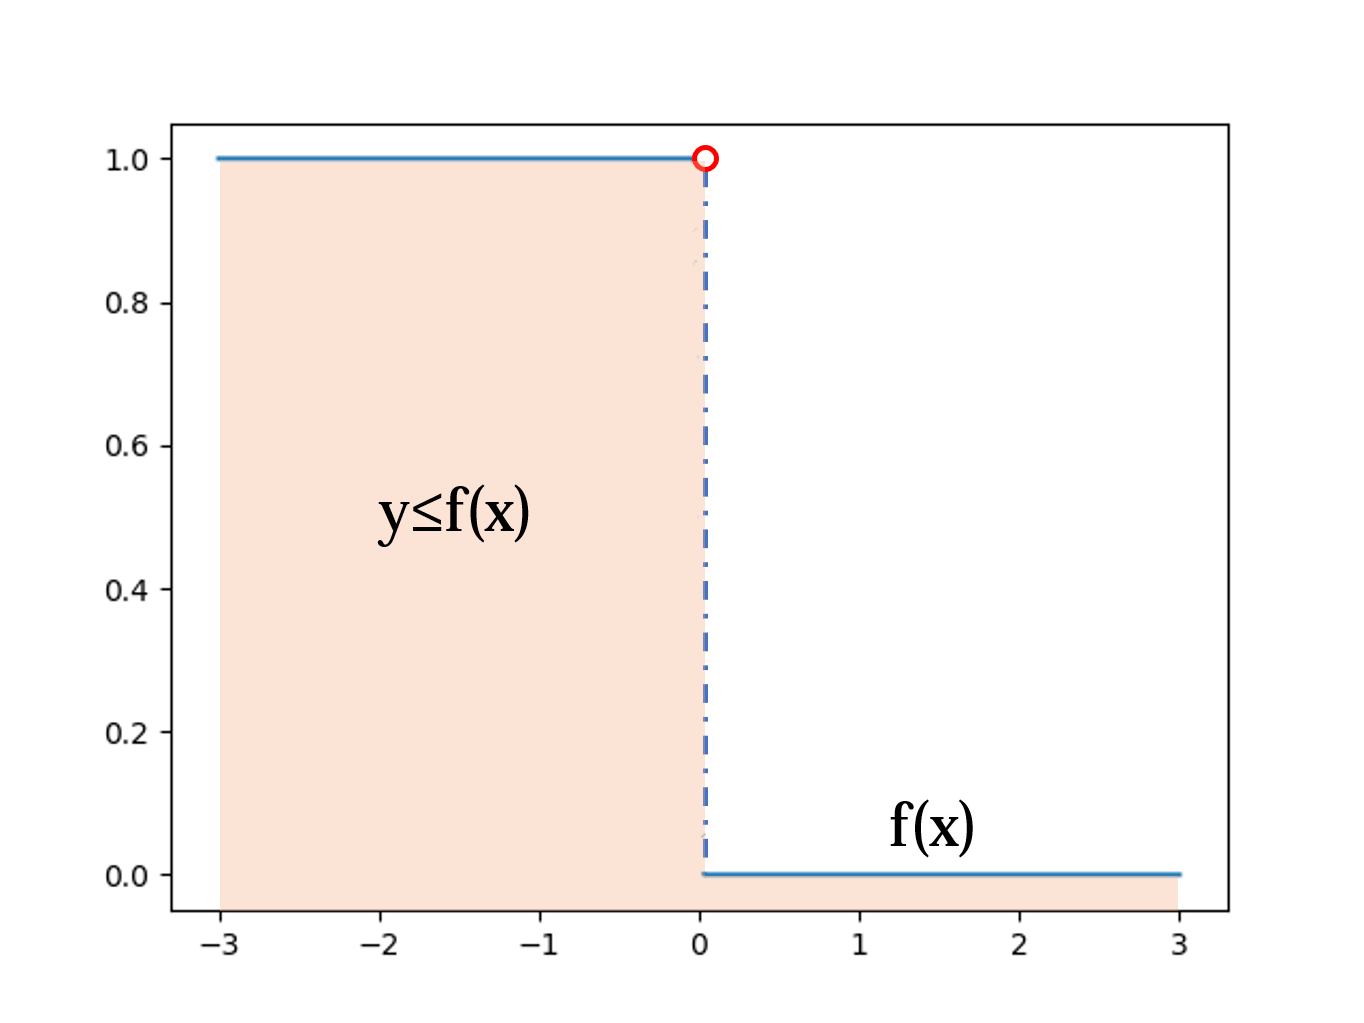
\includegraphics[scale=0.3]{math90.png}
    \end{center}
    %\caption{figure de F}
\end{figure}
F n'est pas un fermé de $(\mathbb{R}^2,\Vert\cdot\Vert_1)$. En fait, on peut définir une suite $((x_n,y_n))_{n \in \mathbb{N}^*}$ telle que 
$\forall n \in \mathbb{N}$, $(x_n,y_n)=(-2^{-n},1)$. Pour tout $n \in \mathbb{N}$, on a $x_n <0$, donc $f(x_n)=1\geq y_n$, donc $(x_n,y_n) \in F$. 

Mais $(x_n,y_n) \xrightarrow[n \to +\infty]{}(0,1) \notin F$, donc \fbox{F n'est pas fermé} 
\subsection{}
On note 
$$
P=F\cup \{(0,y),y\in ]0,1]\}
$$
\begin{itemize}
    \item On va montrer P est un fermé de $(\mathbb{R}^2,\Vert\cdot\Vert_1)$. 
    
    Soit $(x_n,y_n)_{n \in \mathbb{N}}$ de $P$ qui converge dans $\mathbb{R}^2$, alors il existe $(x,y) \in \mathbb{R}^2$ tel que $(x_n,y_n) \xrightarrow[n \to +\infty]{}(x,y)$, 
    donc on a $\Vert(x_n,y_n),(x,y)\Vert _1 \xrightarrow[n \to +\infty]{}0$, donc $x_n\xrightarrow[n \to +\infty]{}x$, $y_n\xrightarrow[n \to +\infty]{}y$
    \begin{itemize}
        \item Si $x<0$, on peut prendre $\epsilon=-\frac{x}{2}>0$, alors il existe $N_1 \in \mathbb{N}$ tel que $\forall n \geq N_1$, $|x_n-x|\leq \epsilon=-\frac{x}{2}$. 
        c'est à dire soit $n \geq N_1$, $x_n\leq \frac{x}{2}<0$, donc $y_n\leq f(x_n)=1$. On a donc $y_n \xrightarrow[n \to \infty]{}y\leq 1=f(x)$, donc $(x,y) \in P$
        \item Si $x>0$, on peut prendre $\epsilon=\frac{x}{2}>0$, alors il existe $N_2 \in \mathbb{N}$ tel que $\forall n \geq N_2$, $|x_n-x|\leq \epsilon=\frac{x}{2}$. 
        c'est à dire soit $n \geq N_2$, $x_n \geq \frac{x}{2}>0$, donc $y_n\leq f(x_n)=0$. On a donc $y_n \xrightarrow[n \to \infty]{}y\leq 0=f(x)$, donc $(x,y) \in P$
        \item Si $x=0$, car $\forall n \in \mathbb{N}$, $y_n \leq f(x_n)\leq 1$, donc $y_n \xrightarrow[n \to +\infty]{} y \leq 1$, donc $(x,y) \in P$
    \end{itemize}
    En tout cas, on a $(x,y)\in P$, donc $P$  est un fermé de $(\mathbb{R}^2,\Vert\cdot\Vert_1)$
    \item Puisque $F \subset P$, donc $\overline{F} \subset \overline{P}=P$ comme $P$ est un fermé de $(\mathbb{R}^2,\Vert\cdot\Vert_1)$
    \item Soit $(x,y)\in P$, on peut toujours trouver une suite $(x_n,y_n)_{n \in \mathbb{N}}$ de F qui converge vers $(x,y)$
    \begin{itemize}
        \item Si $x=0$, on a $y \leq 1$, on pose $\forall n \in \mathbb{N}$, $x_n=-2^{-n}<0$, $y_n=y$, donc soit $n \in \mathbb{N}$, $y_n \leq f(x_n)=1$, donc $(x_n,y_n) \in F$, et on a $\Vert(x_n,y_n),(x,y)\Vert_1=2^{-n}\xrightarrow[n \to +\infty]{}0$, 
        donc $(x,y)$ est la limite d'une suite de $F$, donc $(x,y) \in \overline{F}$
        \item Si $x>0$, on a $y \leq f(x)=0$, on pose $\forall n \in \mathbb{N}$, $x_n=x+2^{-n}>0$, $y_n=y$, donc soit $n \in \mathbb{N}$, $y_n \leq f(x_n)=0$, donc $(x_n,y_n) \in F$, et on a $\Vert(x_n,y_n),(x,y)\Vert_1=2^{-n}\xrightarrow[n \to +\infty]{}0$, 
        donc $(x,y)$ est la limite d'une suite de $F$, donc $(x,y) \in \overline{F}$
        \item Si $x<0$, on a $y \leq f(x)=1$, on pose $\forall n \in \mathbb{N}$, $x_n=x-2^{-n}<0$, $y_n=y$, donc soit $n \in \mathbb{N}$, $y_n \leq f(x_n)=1$, donc $(x_n,y_n) \in F$, et on a $\Vert(x_n,y_n),(x,y)\Vert_1=2^{-n}\xrightarrow[n \to +\infty]{}0$, 
        donc $(x,y)$ est la limite d'une suite de $F$, donc $(x,y) \in \overline{F}$
    \end{itemize}
    On a $\forall (x,y) \in P$, $(x,y) \in \overline{F}$, donc $P \subset \overline{F}$
\end{itemize}
Finalement, on a 
$$
\boxed{\overline{F}=P=F\cup \{(0,y),y\in ]0,1]\}}
$$





\end{document}